\documentclass[12pt,a4paper,openright,twoside]{book}
\usepackage[utf8]{inputenc}
\usepackage{disi-thesis}
\usepackage{code-lstlistings}
\usepackage{notes}
\usepackage{shortcuts}
\usepackage{float}
% \usepackage{acronym}

\school{\unibo}
\programme{Corso di Laurea in Ingegneria e Scienze Informatiche}
\title{OpenGL e Vulkan: un caso di studio}
\author{Palazzini Luca}
\date{\today}
\subject{Computer Graphics}
\supervisor{Prof.ssa Damiana Lazzaro}
\session{I}
\academicyear{2024-2025}

% Definition of acronyms
% \acrodef{API}{Application Programming Interface}
% \acrodef{PBR}{Physically Based Rendering}
% \acrodef{CPU}{Central Processing Unit}
% \acrodef{GPU}{Graphical Processing Unit}

\mainlinespacing{1.241}

\begin{document}

\frontmatter\frontispiece

% TODO: Write abstract
\begin{abstract}	
   Max 2000 characters, strict.
\end{abstract}

% TODO: Write dedication (optional)
\begin{dedication}
   Optional. Max a few lines.
\end{dedication}

% Table of contents
\tableofcontents
\listoffigures
\lstlistoflistings

% Main content
\mainmatter

%----------------------------------------------------------------------------------------
\chapterWithoutNumber{Introduzione}
\label{chap:introduzione}
%----------------------------------------------------------------------------------------

Negli ultimi anni, il campo della grafica computazionale ha visto un'evoluzione significativa delle \emph{Graphics APIs}
verso modelli di programmazione più vicini all'hardware e orientati alle alte prestazioni.
Il contributo principale di questo lavoro consiste nello sviluppo di un motore di rendering modulare che consente
un confronto controllato tra backend OpenGL e Vulkan, con l'obiettivo di analizzarne le differenze prestazionali e architetturali.
Il confronto si concentra in particolare sull'impatto del multithreading in Vulkan rispetto al modello single-thread
tipico di OpenGL, analizzando come la differente gestione della pipeline grafica influisca sulle prestazioni complessive.
L'obiettivo principale del lavoro è progettare e sviluppare un motore di rendering scritto in \emph{C++23},
in grado di operare sia con OpenGL 4.6 sia con Vulkan 1.4. \\
Il motore implementa un approccio di tipo \emph{deferred rendering}, supporta materiali Physically Based Rendering (PBR),
luci direzionali, puntuali e spot, e include ulteriori passaggi di rendering per particelle e oggetti di debug.
L'architettura segue un paradigma orientato agli oggetti, integrando librerie e framework comuni.
L'obiettivo sperimentale è valutare, a parità di contenuto e condizioni di rendering, l'efficienza delle due API
in termini di:
\begin{itemize}
   \item tempo medio per frame e frame rate;
   \item utilizzo della CPU e della GPU.
\end{itemize}
Il progetto è stato sviluppato con un approccio incrementale, secondo cicli iterativi di implementazione e validazione.
Il motore adotta una struttura modulare che separa la logica di rendering dalla gestione della scena, così da consentire
il confronto diretto tra i due backend.
I test prestazionali sono stati condotti su una scena principale: la cattedrale di Sponza~\cite{sponza_original,sponza_intel2022},
utilizzando diversi hardware, variando numero di luci e \emph{particle systems}, per misurare in modo oggettivo i benefici derivati
dal parallelismo offerto da Vulkan.

\paragraph{Struttura della tesi}
La struttura della tesi è la seguente:
\begin{itemize}
   \item Il \textbf{Capitolo 1} introduce i concetti fondamentali relativi al rendering, alle API grafiche moderne e alle tecniche PBR e deferred rendering;
   \item Il \textbf{Capitolo 2} analizza i requisiti del progetto e le scelte progettuali alla base del motore sviluppato;
   \item Il \textbf{Capitolo 3} descrive l'architettura del sistema e i principali componenti software;
   \item Il \textbf{Capitolo 4} illustra l'implementazione e mostra esempi di codice e schermate del motore in funzione;
   \item Il \textbf{Capitolo 5} presenta la valutazione sperimentale, i risultati delle misure e la loro analisi critica.
\end{itemize}

%----------------------------------------------------------------------------------------
\chapter{Fondamenti Teorici}
\label{chap:fondamenti-teorici}
%----------------------------------------------------------------------------------------
\noindent
Questo capitolo fornisce il quadro teorico necessario alla comprensione del lavoro svolto.
Vengono introdotti i concetti fondamentali relativi alla pipeline di rendering,
analizzando le differenze tra i principali approcci utilizzati nei motori grafici moderni,
in particolare il \emph{forward rendering} e il \emph{deferred rendering}.
Segue un approfondimento sui principi del \emph{Physically Based Rendering} (PBR),
che costituisce la base fisica dei modelli di illuminazione implementati nel motore sviluppato.
Infine, vengono presentate le due API grafiche oggetto dello studio, OpenGL e Vulkan,
e le principali librerie di supporto utilizzate nel progetto.
L'obiettivo del capitolo è fornire al lettore una visione d'insieme dei fondamenti teorici e tecnologici
su cui si basa l'intero lavoro sperimentale.

\section{Pipeline di Rendering}
Una pipeline di rendering è una sequenza di fasi che trasforma la rappresentazione tridimensionale di una scena in
un'immagine bidimensionale visualizzabile sullo schermo. Ogni fase elabora i dati provenienti dalla precedente,
passando progressivamente da una descrizione geometrica ad una descrizione visiva.
Nelle API moderne come OpenGL e Vulkan, la pipeline grafica è composta da una serie di stadi programmabili:
elaborazione dei vertici, assemblaggio dei primitivi, rasterizzazione, shading dei frammenti e scrittura nel
\emph{framebuffer}~\ref{fig:rendering-pipeline-overview}.
Nello stadio di elaborazione dei vertici, ogni punto della geometria viene trasformato nello spazio di proiezione,
mentre nello stadio dei frammenti viene calcolato il colore finale di ciascun pixel tenendo conto della luce e delle
proprietà del materiale.
\begin{figure}[H]
   \centering
   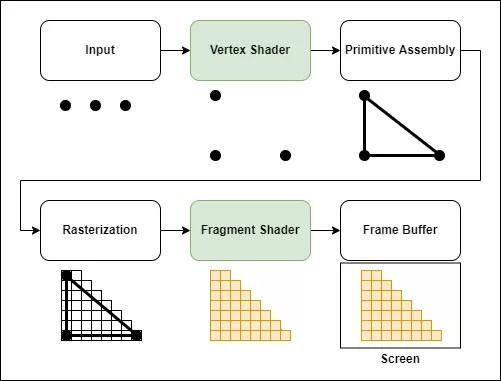
\includegraphics[width=.8\linewidth]{figures/rendering_pipeline_overview.png}
   \caption{Stadi di una pipeline di rendering.}
   \label{fig:rendering-pipeline-overview}
\end{figure}
Il processo di rendering di una scena tridimensionale può essere realizzato attraverso approcci differenti,
ognuno con vantaggi e limiti specifici. I due modelli principali sono il \emph{forward rendering} e il
\emph{deferred rendering}, che differiscono per il modo in cui gestiscono il calcolo dell'illuminazione e la
composizione finale dell'immagine.
Il rendering di una scena tridimensionale trasforma modelli matematici di oggetti e luci in un'immagine bidimensionale,
seguendo diverse pipeline, ciascuna con specifici vantaggi e limiti.
Nel \emph{forward rendering}, ogni oggetto della scena viene renderizzato direttamente con tutte le luci che lo influenzano.
Durante il passaggio di rendering, per ogni frammento vengono calcolati il colore finale e il contributo luminoso
di ciascuna sorgente, con il risultato che il numero di calcoli cresce proporzionalmente al numero di luci.
Questo metodo è relativamente semplice da implementare, ma può diventare inefficiente in scene complesse, dove molte
luci influenzano simultaneamente la stessa area. Tuttavia, rimane ancora oggi una soluzione adatta a contesti con un
numero limitato di luci dinamiche o in applicazioni dove la compatibilità e la semplicità di implementazione sono prioritarie.
Il \emph{deferred rendering}, invece, suddivide il processo di rendering in più passaggi. Nel primo, chiamato
\emph{geometry pass}, vengono memorizzate nei cosiddetti \emph{G-buffer} le informazioni geometriche necessarie,
come la posizione dei punti \(\mathbf{P}\), le normali delle superfici \(\mathbf{N}\) e le proprietà dei materiali
(albedo \(A\), roughness \(r\), metallic \(m\), normal map \(\mathbf{N}\), ambient occlusion AO).
\begin{figure}[H]
   \centering
   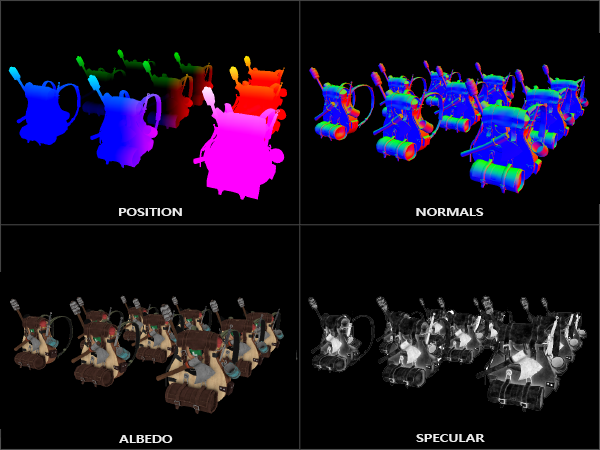
\includegraphics[width=.8\linewidth]{figures/g_buffer_example.png}
   \caption{Esempio di G-buffer in una pipeline di deferred rendering da \cite{learnopengl}.}
   \label{fig:g-buffer-example}
\end{figure}
Nel secondo passaggio, denominato \emph{lighting pass}, l'illuminazione viene calcolata utilizzando i dati salvati
nei buffer~\ref{fig:g-buffer-example}, evitando di dover eseguire nuovamente le trasformazioni geometriche per ogni
luce. L'equazione generale per il colore finale di un frammento è:
\begin{align*}
C_{\text{final}} = \sum_{i=1}^{N_\text{luci}} L_i(\mathbf{P}, \mathbf{N}) \cdot f_r(\mathbf{V}, \mathbf{L}_i, \mathbf{N})
\end{align*}
dove \(L_i\) è il contributo della luce i-esima e \(f_r\) è la funzione di BRDF utilizzata per il materiale del frammento.
Questo approccio permette di gestire un numero elevato di luci in modo più efficiente, rendendolo particolarmente
indicato per applicazioni moderne e motori di gioco con scenari complessi~\ref{fig:deferred-pipeline-example}.
\begin{figure}[H]
   \centering
   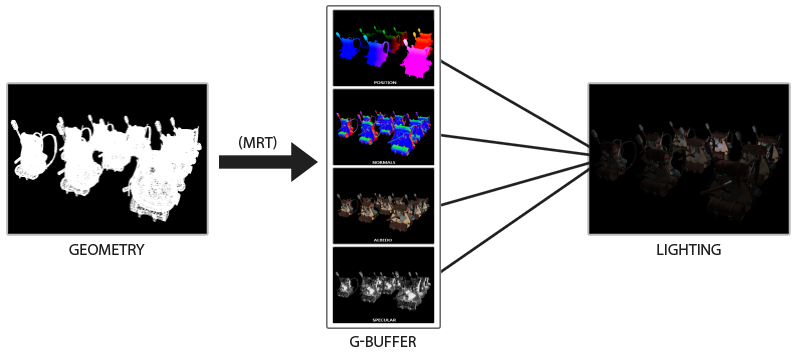
\includegraphics[width=.8\linewidth]{figures/deferred_pipeline_example.png}
   \caption{Schema generale della pipeline di deferred rendering da \cite{learnopengl}.}
   \label{fig:deferred-pipeline-example}
\end{figure}
Il motore sviluppato per questa tesi adotta una pipeline di tipo \emph{deferred}, in quanto offre una base più
flessibile per l'analisi delle prestazioni e per l'integrazione di tecniche di illuminazione avanzate.
Le tecniche di illuminazione descritte nelle sezioni successive, in particolare il Physically Based Rendering,
si integrano con tale pipeline per ottenere una resa fisicamente plausibile dei materiali.

\section{Physically Based Rendering (PBR)}
Il \emph{Physically Based Rendering} (PBR) fornisce un modello matematico per simulare il comportamento reale
della luce quando interagisce con una superficie. Si basa sulla \emph{Legge della Conservazione dell'Energia}
e sull'ipotesi che la luce riflessa o assorbita da un materiale dipenda dalle proprietà fisiche microscopiche
della sua superficie.

\subsection*{Equazione di Rendering}
L'illuminazione totale uscente da un punto $p$ in direzione di vista $\omega_o$ è data da:
\begin{align*}
L_o(p,\omega_o) = \int_{\Omega} f_r(p,\omega_i,\omega_o) \, L_i(p,\omega_i)\, (\mathbf{n}\cdot\omega_i)\,d\omega_i
\end{align*}
\noindent
Qui:
\begin{itemize}
    \item $L_o$ è la radiance uscente, cioè la luce che lascia la superficie verso l'osservatore;
    \item $L_i$ è la radiance incidente, cioè la luce che arriva sulla superficie da una direzione $\omega_i$;
    \item $f_r$ è la funzione di riflettanza bidirezionale (BRDF), che definisce come la luce viene riflessa in base alla direzione incidente e a quella di uscita;
    \item $(\mathbf{n}\cdot\omega_i)$ rappresenta il fattore geometrico di Lambert, cioè quanto la luce è "efficace" in base all'angolo di incidenza.
\end{itemize}
In parole semplici, questa equazione somma tutta la luce incidente sulla superficie pesata da come il materiale
la riflette verso l'occhio dell'osservatore.

\subsection*{Modello Cook-Torrance}
Il modello più diffuso nel PBR è il \emph{Cook-Torrance microfacet model}, che rappresenta la superficie come un insieme
di microfacets inclinati. Ogni microfacet riflette la luce secondo la legge di Fresnel, e la distribuzione delle
loro inclinazioni determina l'aspetto speculare della superficie.
La BRDF si scrive come:
\begin{align*}
f_r(\omega_i,\omega_o) = k_d \frac{A}{\pi} +
k_s \frac{D(\mathbf{n},\mathbf{h})\,F(\omega_o,\mathbf{h})\,G(\omega_i,\omega_o,\mathbf{n})}
{4(\mathbf{n}\cdot\omega_i)(\mathbf{n}\cdot\omega_o)}
\end{align*}
\noindent
Qui il primo termine $k_d \frac{A}{\pi}$ rappresenta la riflessione diffusa lambertiana, responsabile della componente di
colore percepita indipendentemente dall'angolo di vista.
Il secondo termine descrive la riflessione speculare dovuta alla micro-geometria della superficie. In particolare:
\begin{itemize}
    \item $D(\mathbf{n},\mathbf{h})$ è la \emph{Normal Distribution Function} (NDF), che definisce la distribuzione statistica
    dell'orientazione dei microfacets. Controlla la concentrazione del riflesso speculare.
    \item $F(\omega_o,\mathbf{h})$ è il termine di \emph{Fresnel}, che determina la quantità di luce riflessa in funzione
    dell'angolo tra osservatore e microfacet. Governa la crescita del riflesso a incidenti radenti.
    \item $G(\omega_i,\omega_o,\mathbf{n})$ è il termine di \emph{geometrical attenuation}, che modella l'auto-occlusione:
    microfacets possono bloccare la luce incidente o riflessa.
\end{itemize}
Il vettore metà $\mathbf{h} = \frac{\omega_i+\omega_o}{\|\omega_i+\omega_o\|}$ rappresenta la direzione intermedia
tra luce e osservatore, usata per calcolare la riflessione speculare.

\subsection*{Normal Distribution Function (NDF)}
$D(\mathbf{n},\mathbf{h})$ descrive la densità dei microfacets orientati verso la direzione $\mathbf{h}$.  
Un modello comune è il GGX (Trowbridge-Reitz):
\begin{align*}
D_{\text{GGX}}(\mathbf{n},\mathbf{h},r) =
\frac{r^2}
{\pi \big[(\mathbf{n}\cdot\mathbf{h})^2(r^2-1)+1\big]^2}
\end{align*}
\noindent
In pratica, $r$ (roughness) controlla quanto "liscia" o "ruvida" appare la superficie: valori bassi concentrano gli
highlight speculari, valori alti li diffondono e ammorbidiscono.

\subsection*{Fresnel Term}
$F(\omega_o,\mathbf{h})$ rappresenta la variazione dell'intensità della riflessione in base all'angolo di incidenza.
Il modello di Schlick fornisce una buona approssimazione:
\begin{align*}
F(\omega_o,\mathbf{h}) = F_0 + (1 - F_0)(1 - \omega_o\cdot\mathbf{h})^5
\end{align*}
\noindent
Qui, $F_0$ è la riflettanza a incidenza normale (tipicamente 0.04 per dielettrici, uguale al colore del
metallo per metallici).
Questo termine genera l'effetto noto in grafica come "specular highlight più intenso ai bordi".

\subsection*{Geometric Term}
$G(\omega_i,\omega_o,\mathbf{n})$ tiene conto dell'auto-occlusione dei microfacets, cioè che alcuni microfacets
possono bloccare la luce di altri:
\begin{align*}
G(\omega_i,\omega_o,\mathbf{n}) = G_1(\omega_i,\mathbf{n}) \, G_1(\omega_o,\mathbf{n})
\end{align*}
\begin{align*}
G_1(\omega,\mathbf{n}) =
\frac{2(\mathbf{n}\cdot\omega)}
{(\mathbf{n}\cdot\omega) + \sqrt{r^2 + (1-r^2)(\mathbf{n}\cdot\omega)^2}}
\end{align*}
In parole semplici, quando la luce colpisce la superficie a un angolo basso o quando la vista è laterale, parte
della luce viene "nascosta" dai microfacets, riducendo la riflessione percepita~\ref{fig:pbr-material-render}.

\subsection*{Equazione completa di illuminazione}
Combinando i termini precedenti, l'illuminazione riflessa diventa:
\begin{align*}
L_o(p,\omega_o) =
\int_{\Omega}
\left(
k_d\frac{A}{\pi} +
\frac{D\,F\,G}
{4(\omega_o\cdot\mathbf{n})(\omega_i\cdot\mathbf{n})}
\right)
L_i(p,\omega_i)\,
(\mathbf{n}\cdot\omega_i)\,d\omega_i
\end{align*}
\noindent
Questa integrazione viene valutata in modo approssimato nel rendering in tempo reale tramite
\emph{environment maps}, \emph{prefiltered radiance} e \emph{BRDF lookup tables}.
In pratica, ogni termine della formula corrisponde a un effetto visivo:
\begin{itemize}
    % TODO: Interlinea strano
    \item $k_d A/\pi$ → colore diffuso del materiale;
    \item $D$ → forma e ampiezza dello speculare;
    \item $F$ → intensità speculare in base all'angolo di visuale;
    \item $G$ → riduzione della luce dovuta all'auto-occlusione dei microfacets.
\end{itemize}
\begin{figure}[H]
   \centering
   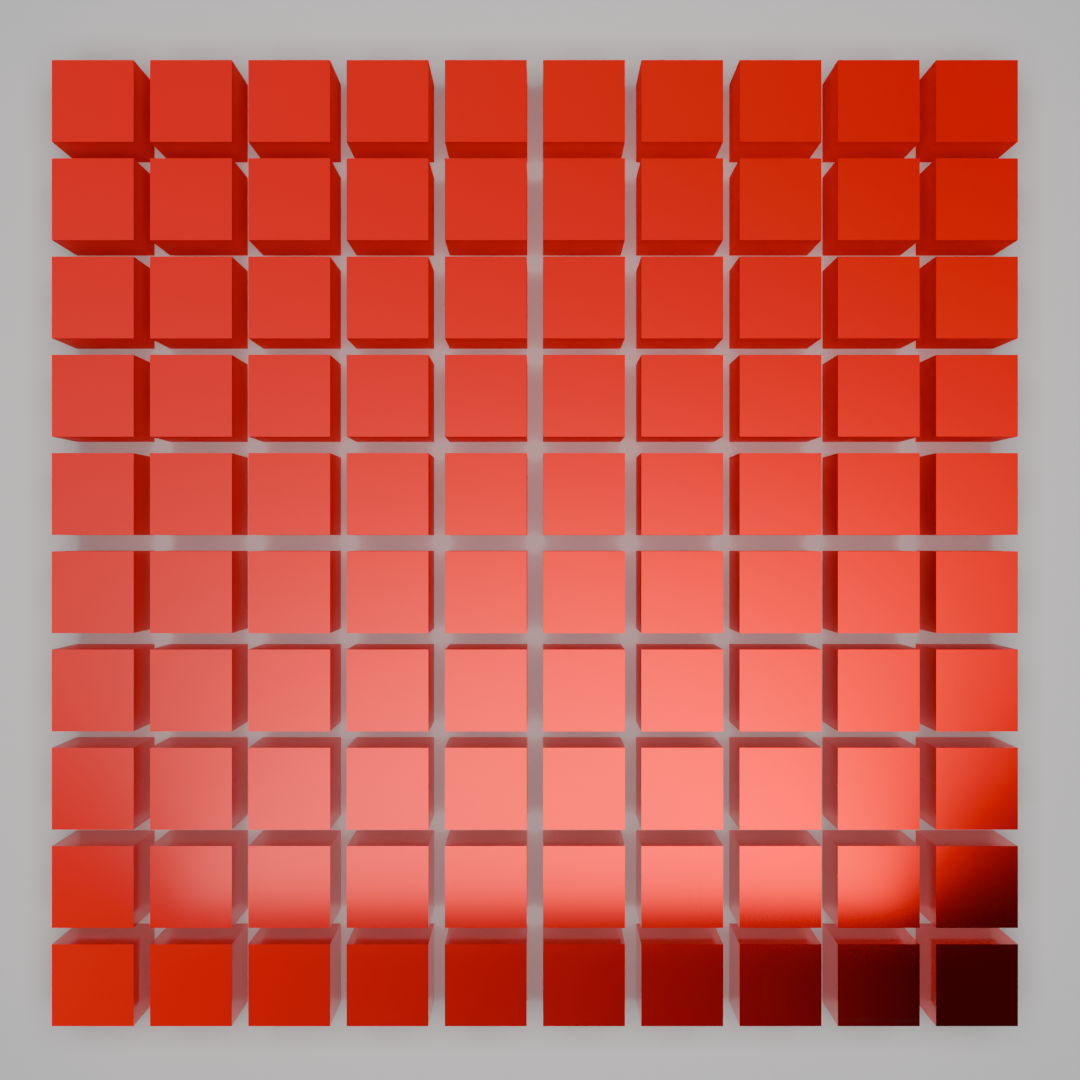
\includegraphics[width=.8\linewidth]{figures/pbr_material_render.png}
   \caption{Array di 10$\times$10 cubi che mostra l'effetto della variazione di roughness (righe) e metalness
      (colonne) sui materiali PBR.}
   \label{fig:pbr-material-render}
\end{figure}
\noindent
L'aumento di roughness disperde la luce, generando highlight più ampi e opachi~\ref{fig:pbr-material-example};
l'aumento del valore metallic incrementa la riflessione speculare e riduce la componente diffusa.
Queste relazioni rendono il PBR un modello coerente e fisicamente plausibile per la rappresentazione
di materiali in ambienti virtuali.
\begin{figure}[H]
   \centering
   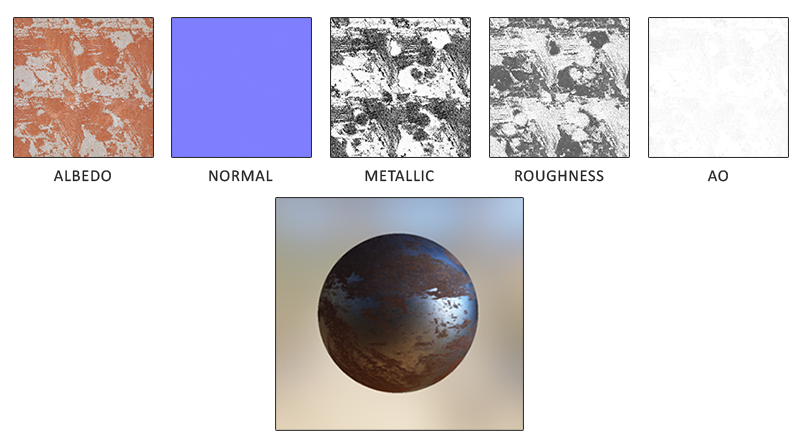
\includegraphics[width=.8\linewidth]{figures/pbr_material_example.png}
   \caption{Esempio di materiale PBR da \cite{learnopengl}.}
   \label{fig:pbr-material-example}
\end{figure}

\section{Graphics API: OpenGL and Vulkan}
OpenGL e Vulkan rappresentano due approcci concettualmente diversi allo sviluppo di applicazioni grafiche. \\
OpenGL è un'API di livello alto che semplifica notevolmente la gestione della pipeline grafica: gran parte del lavoro
legato alla sincronizzazione delle risorse, alla gestione della memoria e alla compilazione dei comandi GPU è affidato
al driver. Questo approccio riduce la complessità dello sviluppo, consentendo di ottenere rapidamente risultati visivi,
ma limita il controllo del programmatore sulle prestazioni, soprattutto in scenari con molte luci e geometrie complesse.
OpenGL opera principalmente in modalità single-thread, affidando al driver l'organizzazione dei comandi su GPU, il che può
generare overhead significativi in applicazioni moderne e multithreaded. \\
Vulkan, al contrario, offre un modello di programmazione a basso livello, dove il programmatore ha il controllo diretto
sulla memoria, sui comandi e sulla sincronizzazione. La pipeline Vulkan richiede la definizione esplicita di tutti i
passaggi di rendering attraverso strutture come \texttt{Render Pass} e \texttt{Command Buffers}, e la gestione della 
sincronizzazione è completamente esplicita mediante \texttt{Semaphore} e \texttt{Fence}. Questo approccio riduce
l'overhead del driver e permette di sfruttare pienamente il multithreading della CPU, rendendo più efficienti
le applicazioni che devono gestire grandi quantità di oggetti e luci in scena. Allo stesso tempo, Vulkan richiede
una conoscenza approfondita dell'architettura hardware e della gestione delle risorse, aumentando la complessità
dello sviluppo rispetto a OpenGL.

\section{Librerie e Strumenti}
Il motore sviluppato utilizza un insieme di librerie open source per la gestione dell'infrastruttura di rendering
e delle funzionalità.
La combinazione di queste librerie ha permesso di ridurre il tempo di sviluppo e concentrarsi sulle differenze
architetturali tra OpenGL e Vulkan.
\begin{itemize}
   \item \textbf{GLFW}: fornisce un'interfaccia multipiattaforma per la creazione di finestre e la gestione dell'input.
      È utilizzata sia per il backend OpenGL che Vulkan;
   \item \textbf{GLAD}: gestisce il caricamento dinamico delle estensioni OpenGL;
   \item \textbf{Vulkan Memory Allocator (VMA)} e \textbf{vk-bootstrap}: semplificano la configurazione e la gestione della memoria
      Vulkan, riducendo la complessità di codice di inizializzazione;
   \item \textbf{glm}: libreria matematica per operazioni su vettori, matrici e trasformazioni 3D;
   \item \textbf{ImGui}: libreria per la costruzione di interfacce grafiche di debug e monitoraggio delle prestazioni in tempo reale;
   \item \textbf{stb\_image}: caricamento di texture in vari formati;
   \item \textbf{ASSIMP}: parsing dei modelli 3D in formato \texttt{.obj} e \texttt{.fbx}.
\end{itemize}

\section{Lavori Correlati}
Diversi studi e progetti hanno analizzato il confronto tra OpenGL e Vulkan, evidenziando vantaggi significativi di
Vulkan in termini di efficienza e parallelismo.
Il \emph{Khronos Group}, nelle specifiche di rilascio e nei documenti ufficiali, evidenzia come Vulkan sia progettata per
minimizzare l'overhead del driver e fornire prestazioni più prevedibili grazie a un controllo esplicito delle risorse e
dell'esecuzione dei comandi \cite{khronos_vulkan_spec,vulkan_overview,google_vulkan_lowoverhead}.
Sul fronte applicativo, motori come \emph{Unreal Engine 5} e \emph{Unity} hanno introdotto backend Vulkan per
ottimizzare la scalabilità su dispositivi moderni, mantenendo al contempo compatibilità con OpenGL su piattaforme legacy.

%----------------------------------------------------------------------------------------
\chapter{Requisiti ed Analisi}
\label{chap:analisi}
%----------------------------------------------------------------------------------------
\noindent
In questo capitolo vengono definiti i requisiti funzionali e non funzionali del motore di rendering 
e analizzate le motivazioni alla base delle scelte progettuali.
L'obiettivo è stabilire un quadro metodologico chiaro che guidi la progettazione e l'implementazione del sistema,
tenendo conto dei vincoli tecnici imposti dalle API e dall'hardware.
Lo sviluppo del motore di rendering oggetto di questo elaborato nasce con l'obiettivo di creare una piattaforma
sperimentale che permetta di confrontare in modo diretto le prestazioni e le differenze architetturali tra
OpenGL e Vulkan.
Dopo aver descritto le funzionalità attese e le caratteristiche qualitative del software,
si discutono i principali vincoli di progetto e le librerie adottate.
Il capitolo si conclude illustrando la strategia di valutazione delle prestazioni,
che costituisce la base per l'analisi comparativa tra OpenGL e Vulkan presentata nei capitoli successivi.
Le analisi svolte guidano le scelte architetturali descritte nei capitoli successivi.

\section{Requisiti funzionali}
Dal punto di vista funzionale, il motore deve essere in grado di gestire l'intero processo di rendering di una
scena tridimensionale complessa, fornendo un'infrastruttura flessibile per la sperimentazione con entrambe le API.
Il primo requisito riguarda la possibilità di selezionare, in fase di avvio, quale backend utilizzare tra OpenGL e
Vulkan. Tale scelta consente di confrontare le due pipeline in modo trasparente, mantenendo invariata la struttura
logica del motore e la scena visualizzata. \\
Il motore deve poi garantire la gestione completa delle risorse grafiche, tra cui modelli tridimensionali, texture e
shader. A tal fine, è stato previsto un sistema di caricamento e caching che consente di ridurre le operazioni ridondanti
e di ottimizzare la condivisione della memoria tra CPU e GPU. Il rendering della scena è realizzato attraverso una
pipeline di tipo \emph{deferred}, scelta per la sua maggiore efficienza nella gestione di un elevato numero di luci
dinamiche. \\
Un ulteriore requisito fondamentale riguarda il supporto al \emph{Physically Based Rendering (PBR)}, che permette
di ottenere una resa realistica dei materiali basandosi su parametri fisici. Il sistema deve inoltre consentire
l'utilizzo di differenti tipologie di luci con parametri configurabili dall'interfaccia di debug. \\
Nel backend Vulkan, il motore deve supportare la generazione multithread dei \texttt{command buffer}, così da sfruttare
in modo più efficiente i core della CPU. Questa caratteristica è essenziale per valutare i benefici del parallelismo
offerto da Vulkan rispetto al modello single-thread di OpenGL. Infine, il motore deve includere una telecamera
controllabile in tempo reale e un'interfaccia grafica basata su ImGui per la visualizzazione delle statistiche di
esecuzione e dei parametri di scena.

\section{Requisiti non-funzionali}
Oltre alle funzionalità previste, il progetto deve rispettare una serie di requisiti non funzionali che ne
determinano la qualità complessiva. L'aspetto più rilevante è quello prestazionale: il motore deve essere in grado
di mantenere un frame rate stabile e prevedibile, anche in presenza di scene complesse. L'efficienza del codice e
la riduzione dell'overhead di CPU sono obiettivi primari, soprattutto nella versione Vulkan. \\
Un altro requisito riguarda la portabilità. Il sistema deve poter essere compilato ed eseguito sia su Windows che su
Linux, senza modifiche sostanziali al codice sorgente. Questo ha orientato la scelta di librerie multipiattaforma
come GLFW per la gestione delle finestre e dell'input, e glm per le operazioni matematiche tridimensionali.
La manutenibilità è stata garantita attraverso una struttura modulare del codice, che separa nettamente la logica di
rendering dalle altre componenti, come la gestione delle risorse o la GUI. Tale separazione consente di estendere il
motore in futuro con nuove tecniche di shading o ulteriori passaggi di rendering, senza introdurre dipendenze
circolari o modifiche invasive. \\
L'affidabilità rappresenta un ulteriore requisito importante. In particolare, è necessario assicurare che le risorse
allocate sulla GPU vengano correttamente rilasciate al termine dell'esecuzione, prevenendo perdite di memoria o crash.
La presenza dell'interfaccia di debug consente inoltre di monitorare in tempo reale l'utilizzo delle risorse e il
tempo di esecuzione dei frame, migliorando la tracciabilità e la diagnosi dei colli di bottiglia.

\section{Vincoli di progetto}
Il progetto è stato sviluppato nel rispetto di alcuni vincoli tecnici legati sia alla piattaforma hardware sia alle
librerie disponibili. Il linguaggio scelto è \textbf{C++23}, che offre un buon compromesso tra efficienza,
astrazione e modernità, consentendo l'utilizzo di costrutti avanzati come le \emph{smart pointer} e le
\emph{range-based loops}. Le API grafiche target sono OpenGL 4.6 e Vulkan 1.4, in modo da garantire compatibilità
con la maggior parte delle GPU moderne. \\
% TODO: Introdurre hardware diversi (testato su piu hardware)
Dal punto di vista hardware, i test sono stati condotti su una configurazione dotata di processore multi-core e GPU
di fascia medio-alta compatibile con le specifiche Vulkan. Le prestazioni sono state misurate in un ambiente hardware
costante per garantire ripetibilità e confrontabilità dei risultati. \\
Il motore si appoggia a un insieme di librerie open source per ridurre il tempo di sviluppo e migliorare la stabilità
del codice. Tra queste rientrano GLFW per la creazione delle finestre, GLAD per il caricamento dinamico delle estensioni
OpenGL, Vulkan Memory Allocator e vk-bootstrap per la gestione semplificata delle risorse Vulkan, ImGui per
l'interfaccia di debug, glm per le operazioni matematiche e ASSIMP per il caricamento dei modelli tridimensionali.
Il sistema di build è basato su CMake, scelto per la sua compatibilità multipiattaforma e l'integrazione con ambienti
di sviluppo moderni. \\
Per delimitare il campo di studio, sono stati esclusi elementi non essenziali all'obiettivo sperimentale, come il
ray tracing, le ombre dinamiche avanzate o il supporto a dispositivi mobili. La ricerca si concentra esclusivamente
sulle differenze di prestazioni e di gestione delle risorse tra le due API, in un contesto di rendering differito
tradizionale.

\section{Strategia di Valutazione}
La valutazione delle prestazioni rappresenta una parte fondamentale di questo lavoro. La strategia adottata prevede
una serie di test ripetibili e controllati, condotti su una scena di riferimento comune: la cattedrale di
Sponza~\cite{sponza_original,sponza_intel2022}, ampiamente utilizzata come benchmark nella letteratura di grafica
computazionale. I test vengono eseguiti con configurazioni identiche per i due backend, variando il numero di luci,
la complessità della scena e il livello di parallelismo della CPU.
Le metriche considerate includono il tempo medio per frame, il frame rate e l'utilizzo medio della CPU e della GPU.
I dati vengono raccolti tramite un sistema di monitoraggio integrato nell'interfaccia di debug, che consente la
registrazione automatica dei risultati per l'analisi successiva.
Ciascun test viene ripetuto più volte per ridurre l'impatto di fattori esterni, come i processi di sistema o
l'oscillazione della frequenza della GPU. I risultati vengono poi confrontati e discussi nel
Capitolo~\ref{chap:valutazione}, dove vengono analizzate le differenze di comportamento tra OpenGL e Vulkan in termini
di efficienza, scalabilità e prevedibilità delle prestazioni.

%----------------------------------------------------------------------------------------
\chapter{Progettazione e Architettura del Sistema}
\label{chap:design}
%----------------------------------------------------------------------------------------
\noindent
In questo capitolo viene presentata l'architettura del motore di rendering sviluppato. Dopo aver definito i requisiti
e analizzato i fondamenti teorici nei capitoli precedenti, il focus qui è sulle scelte progettuali concrete,
l'organizzazione dei moduli e l'interazione tra le componenti principali. Il capitolo descrive sia la struttura
orientata agli oggetti adottata, sia la pipeline di rendering e la gestione delle risorse, con particolare attenzione
alle differenze tra i backend OpenGL e Vulkan.

\section{Panoramica del Sistema}
Il motore è organizzato in moduli principali che cooperano per fornire un sistema modulare e facilmente estendibile. \\
La scena è gestita da un \emph{Scene Manager} che contiene nodi e componenti, tra cui \texttt{TransformComponent},
\texttt{Camera}, \texttt{LightComponent} e \texttt{ParticleSystemComponent}. Il modulo di rendering si occupa di
orchestrare la pipeline grafica, interfacciandosi con i backend OpenGL e Vulkan attraverso l'interfaccia unificata
\texttt{IRenderer}. \\
\lstinputlisting[float,language=C++,label={lst:renderer-factory}]{listings/renderer_factory.cpp}
La gestione delle risorse, inclusi mesh, texture e shader, è centralizzata nel \texttt{ResourceManager}, che utilizza
factory specifiche per ciascun backend.
Il flusso di dati all'interno del motore parte dall'inserimento degli oggetti nella scena, passa attraverso i componenti
della scena, viene trasformato in strutture di dati compatibili con il backend selezionato e infine elaborato dalla
pipeline di rendering~\ref{fig:uml-scene-renderer}. Le metriche di performance sono raccolte dal modulo \texttt{PerformanceLogger} e rese disponibili
tramite \texttt{PerformanceGUI}, consentendo il monitoraggio in tempo reale.
\begin{figure}[H]
   \centering
   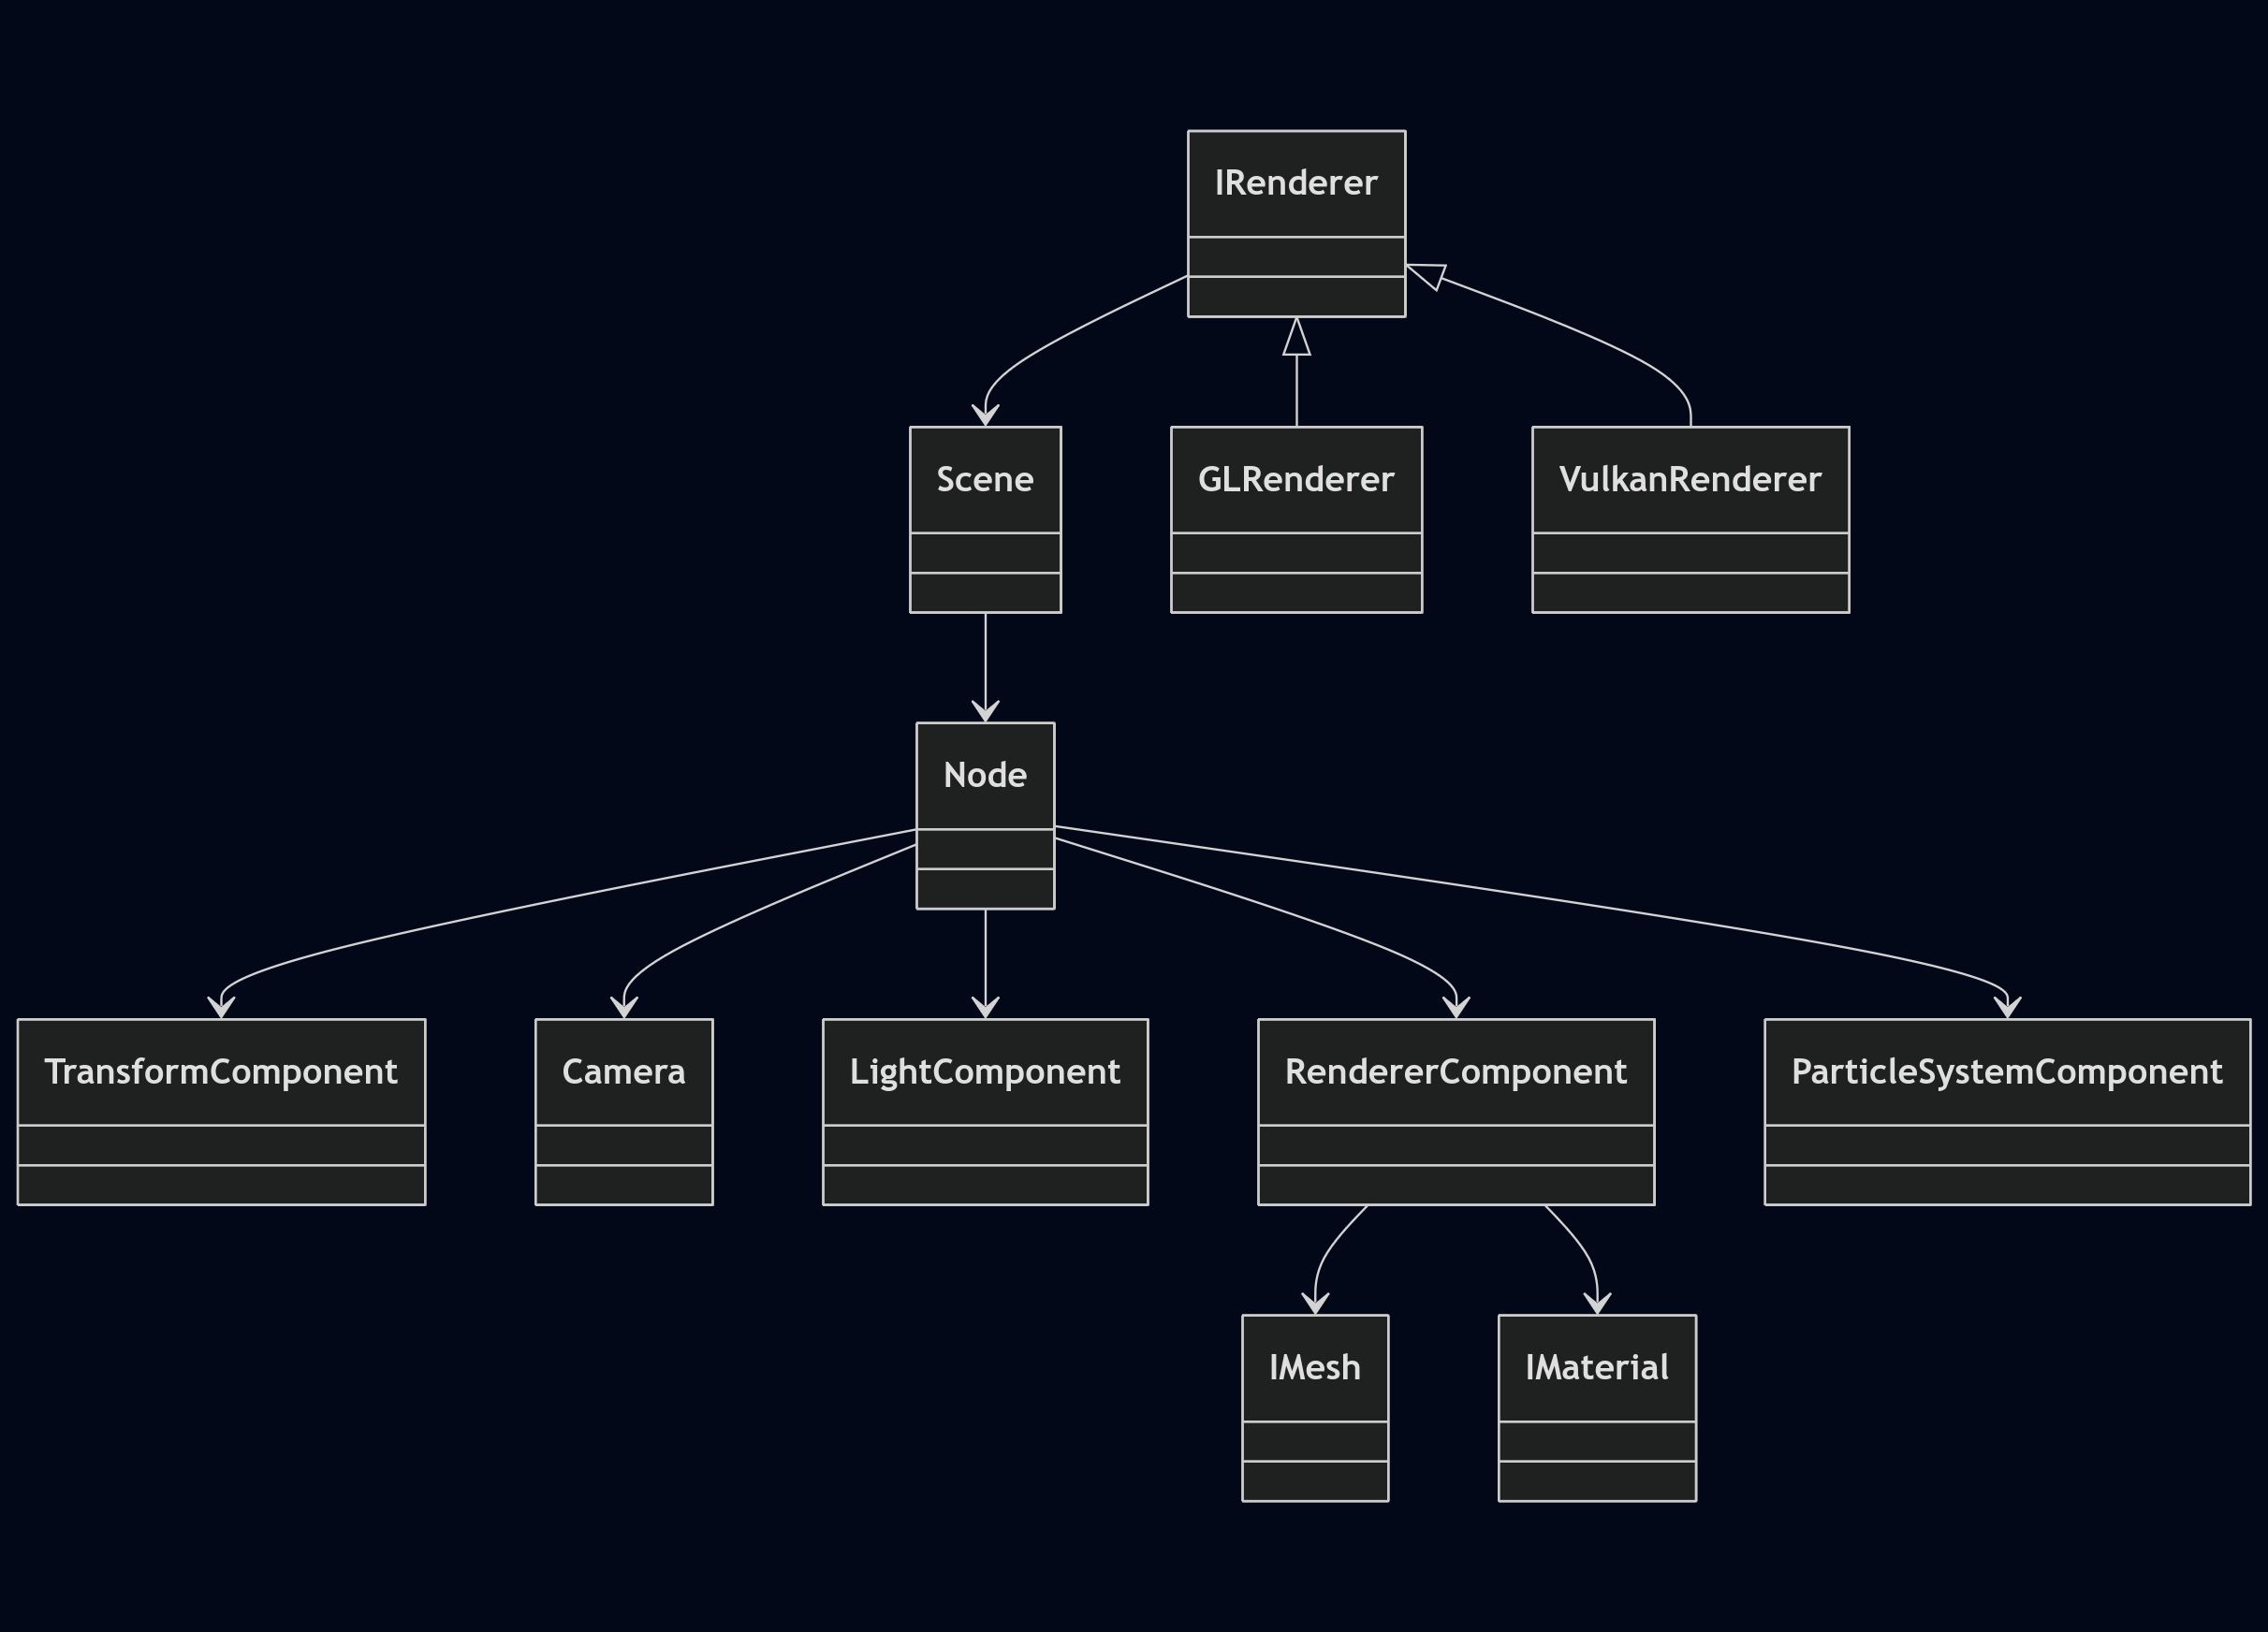
\includegraphics[width=.8\linewidth]{figures/uml_scene_renderer.png}
   \caption{Panoramica delle interazioni fra renderer e la scena.}
   \label{fig:uml-scene-renderer}
\end{figure}

\section{Progettazione Orientata agli Oggetti}
L'architettura si basa su interfacce astratte e classi concrete per separare logica generale e specifiche del backend.
L'interfaccia \texttt{IRenderer} definisce le operazioni principali di inizializzazione, rendering e pulizia delle risorse.
Le implementazioni concrete \texttt{GLRenderer} e \texttt{VulkanRenderer} gestiscono rispettivamente OpenGL e Vulkan,
incapsulando la complessità di ciascun backend e garantendo un'interfaccia unificata al livello superiore.
Le classi legate alla scena, come \texttt{Scene}, \texttt{Node}, \texttt{TransformComponent} e \texttt{LightComponent},
permettono di organizzare gli oggetti in una gerarchia e di propagare trasformazioni e proprietà
di illuminazione~\ref{fig:uml-activity-dynamic-backend}. La gestione dei materiali PBR è realizzata tramite le classi
\texttt{MaterialTemplate} e \texttt{MaterialInstance}, consentendo la definizione di parametri fisicamente plausibili per ogni oggetto.
\begin{figure}[H]
    \centering
    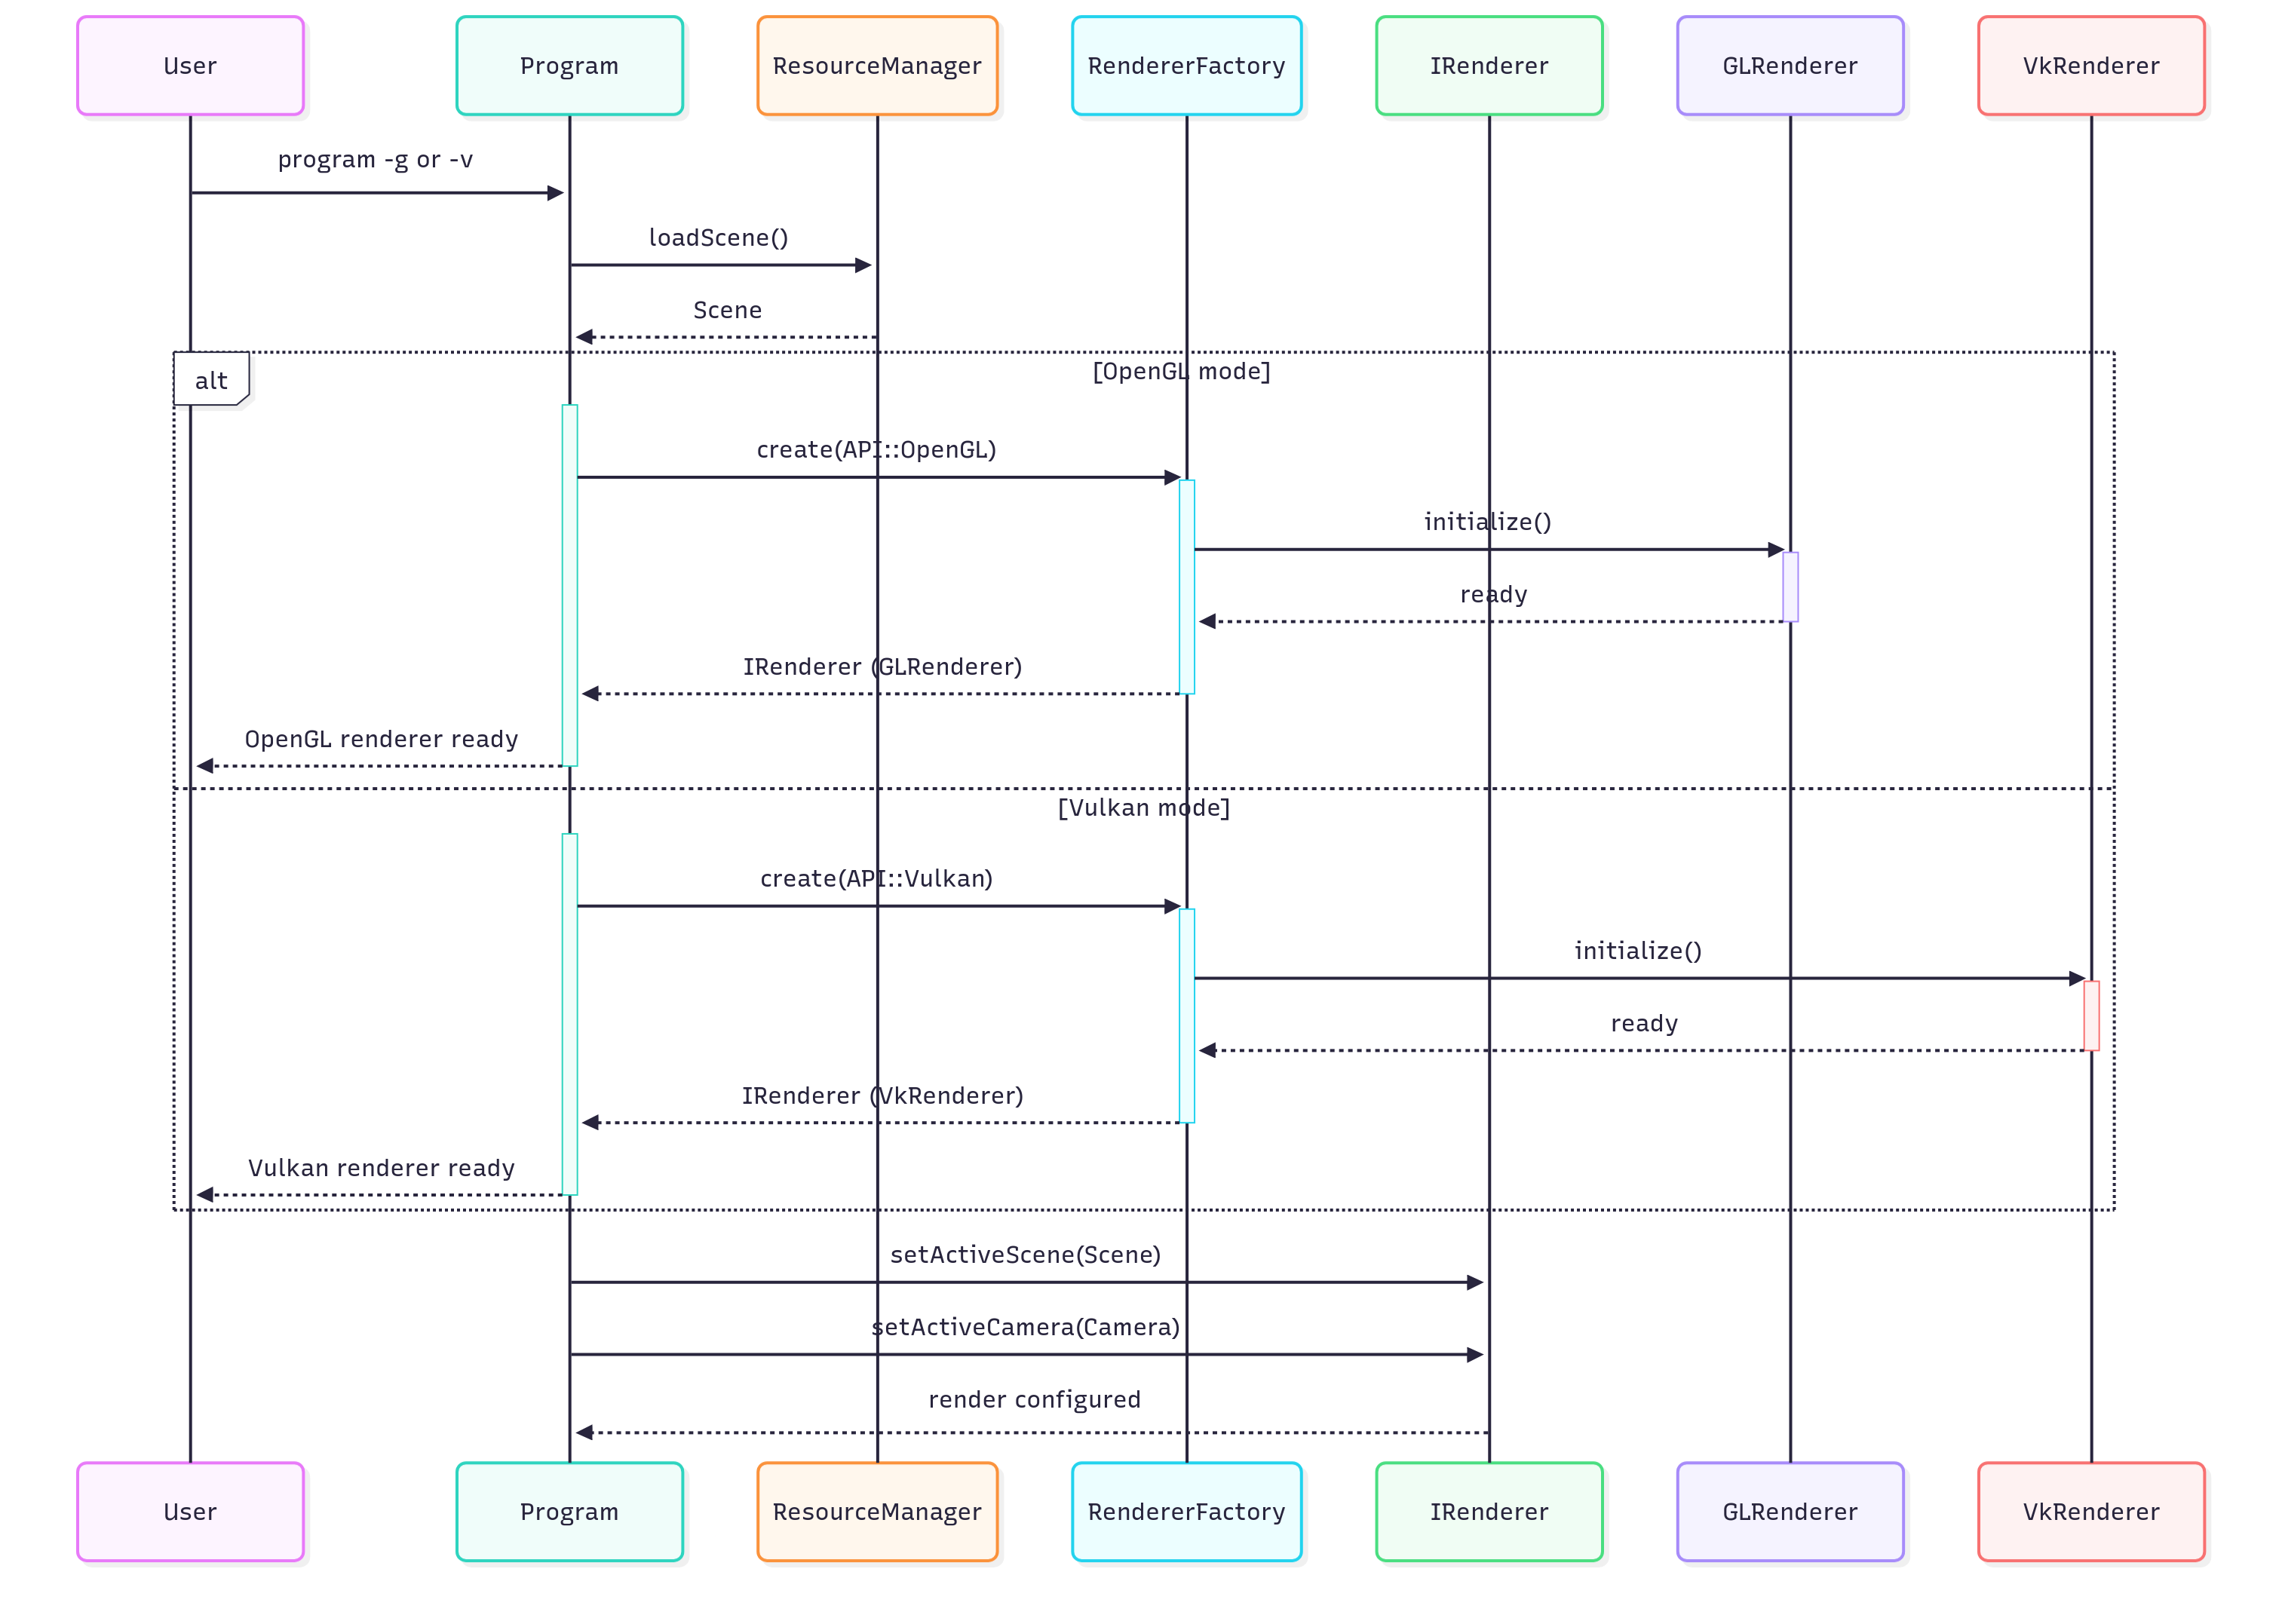
\includegraphics[width=.95\linewidth]{figures/uml_activity_dynamic_backend.png}
    \caption{Selezione dinamica del backend grafico all'avvio.}
    \label{fig:uml-activity-dynamic-backend}
\end{figure}

\section{Architettura del Motore di Rendering}
Il motore separa nettamente la logica di rendering dalla gestione della scena e delle risorse. Nel backend OpenGL,
la sincronizzazione e la gestione delle risorse sono affidate al driver, mentre in Vulkan ogni passaggio richiede controllo
esplicito di buffer, command pool e sincronizzazione tramite \texttt{Semaphore} e \texttt{Fence}. Questa separazione facilita
il confronto diretto tra i due backend senza alterare la logica della scena.
La pipeline di rendering è basata su deferred rendering. Il \emph{geometry pass} popola i G-buffer con informazioni sui
vertici e sui materiali. Il \emph{lighting pass} utilizza queste informazioni per calcolare l’illuminazione, evitando
ricalcoli geometrici e ottimizzando le operazioni per frammento~\ref{fig:g-buffer-textures}. L'oct-encoding delle normali
riduce lo spazio occupato senza perdita significativa di precisione, mentre l’integrazione dei parametri PBR nei canali
texture ottimizza l’uso della memoria GPU.

\section{Pipeline di Deferred Rendering}
Il motore utilizza un approccio di tipo \emph{deferred rendering}, separando la gestione della geometria dalla fase
di illuminazione. Nel primo passaggio, chiamato \emph{geometry pass}, le informazioni sui vertici e sulle proprietà dei
materiali vengono salvate nei G-buffer, mentre nel \emph{lighting pass} l'illuminazione viene calcolata utilizzando
questi dati.
Per il geometry pass, viene utilizzato uno shader GLSL dedicato che calcola le informazioni necessarie per ciascun
frammento della scena. Lo shader scrive nei G-buffer due texture principali:
\begin{itemize}
    \item \texttt{gAlbedo}: canali RGB per il colore diffuso, canale A per l'AO.
    \item \texttt{gNormal}: normali codificate tramite un algoritmo di \emph{oct-encoding} nei canali RG, canale B per roughness, canale A per metallic.
\end{itemize}
\begin{figure}[H]
    \centering
    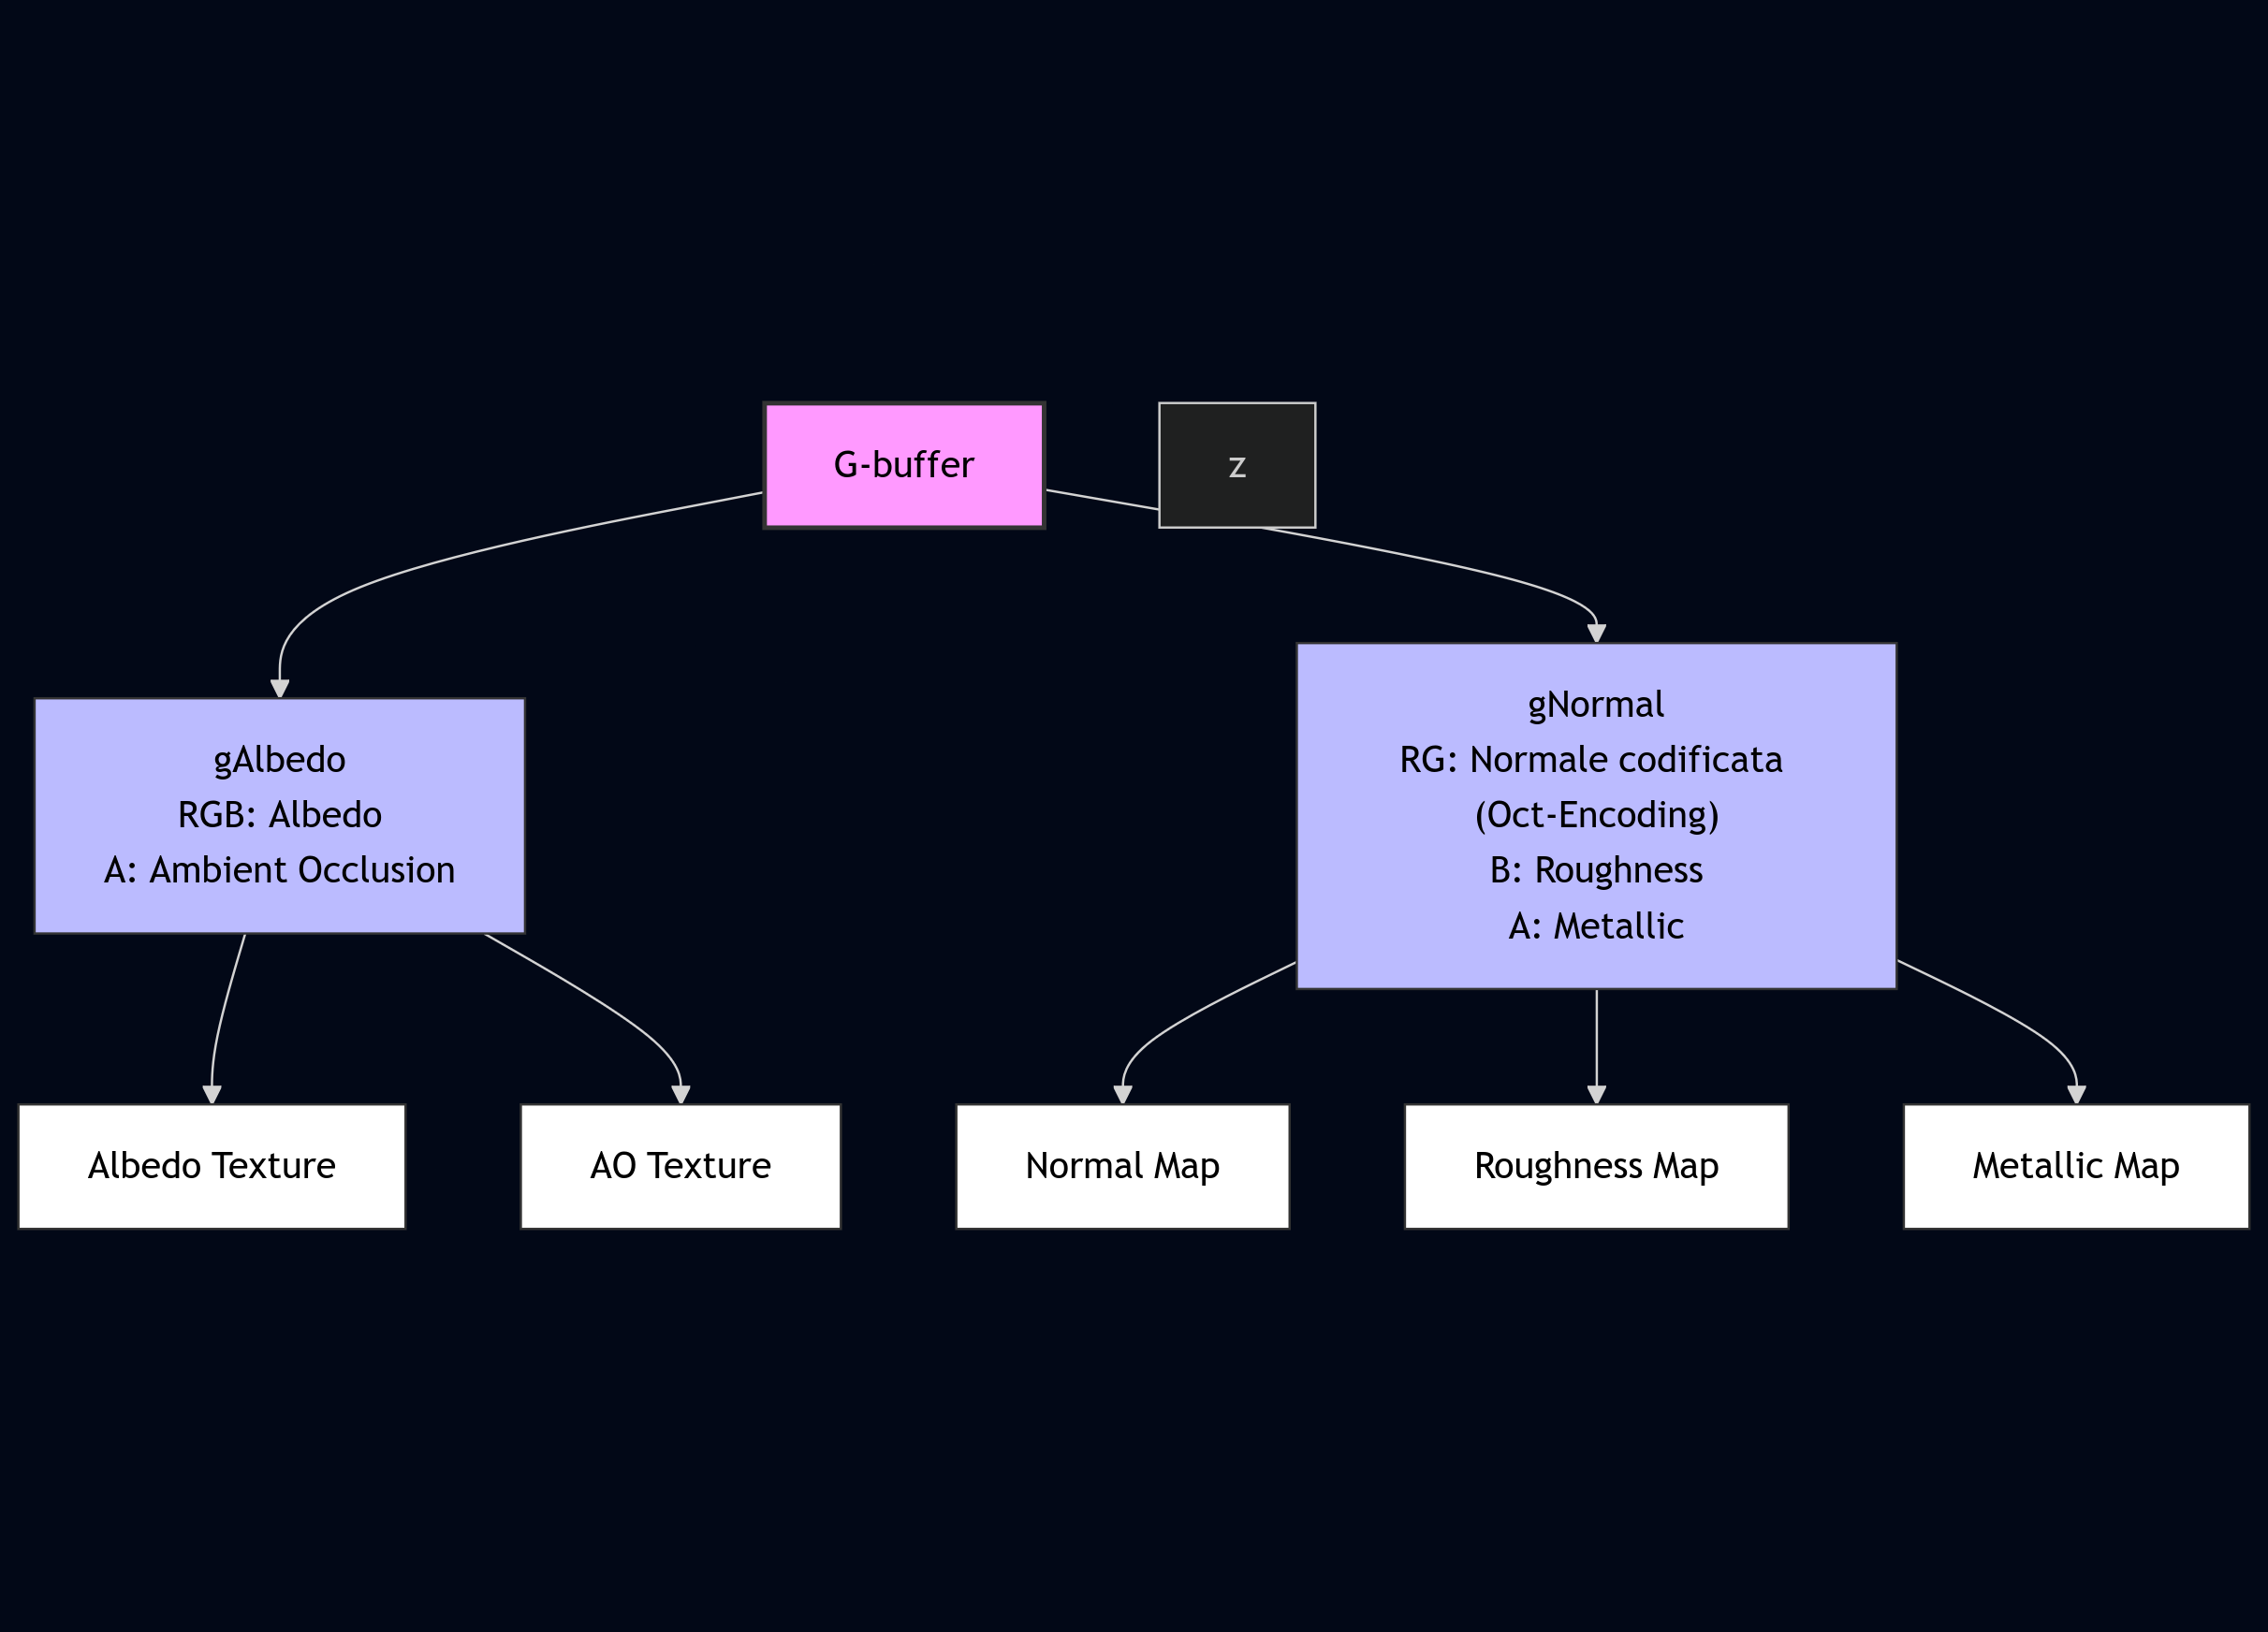
\includegraphics[width=.8\linewidth]{figures/g_buffer_textures.png}
    \caption{Struttura del G-buffer con le texture e i canali utilizzati.}
    \label{fig:g-buffer-textures}
\end{figure}
L'utilizzo dell'\emph{oct-encoding} per le normali permette di comprimere le tre componenti spaziali in due canali,
riducendo lo spazio di memoria richiesto senza perdita significativa di precisione. Inoltre, l'integrazione dei parametri
PBR nei canali non utilizzati della texture (roughness e metallic) ottimizza ulteriormente l'uso della memoria GPU.
Nel passaggio di lighting, il motore legge queste texture e calcola l'illuminazione utilizzando le informazioni PBR
memorizzate, evitando di ricalcolare la geometria e ottimizzando il numero di operazioni per frammento.
La combinazione di queste tecniche garantisce un G-buffer compatto e performante, compatibile sia con OpenGL sia
con Vulkan, mantenendo alta la qualità visiva e minimizzando l'overhead di memoria e banda~\ref{fig:uml-activity-rendering}.
\begin{figure}[H]
    \centering
    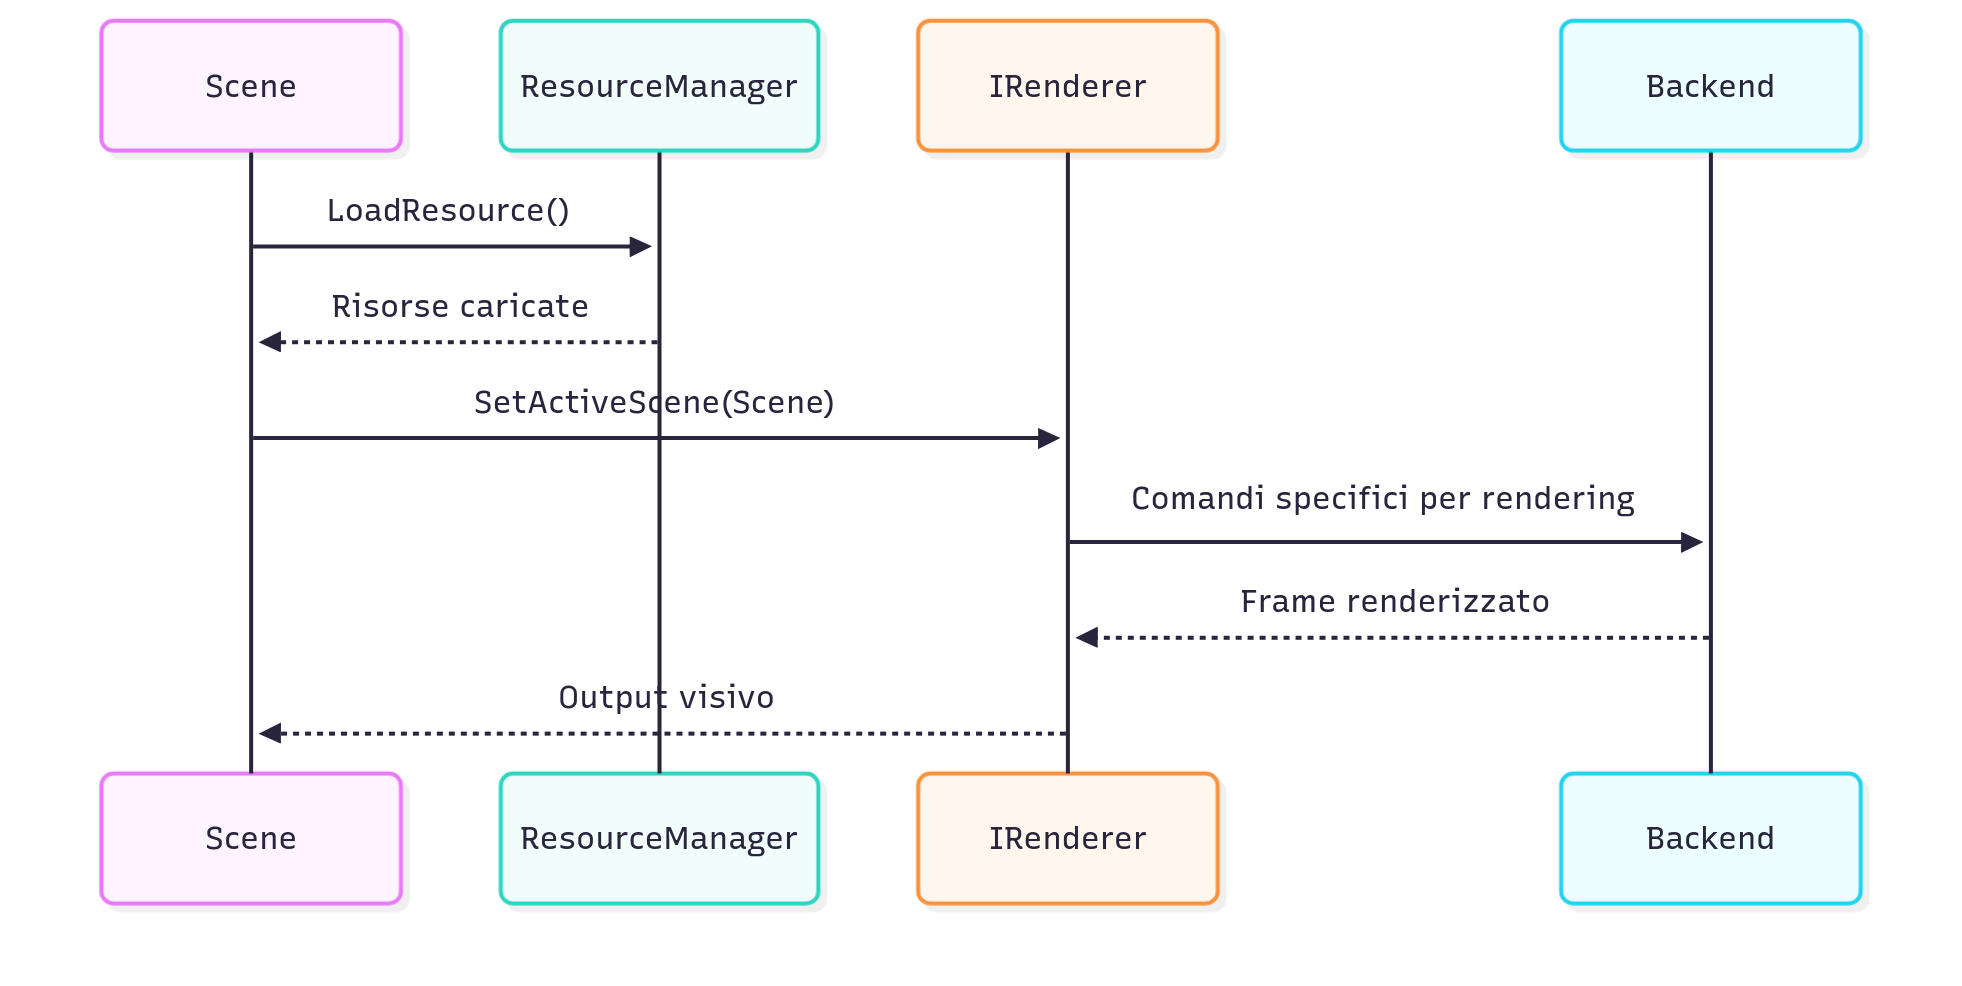
\includegraphics[width=.8\linewidth]{figures/uml_activity_rendering.png}
    \caption{Flusso di rendering della scena attraverso il motore e i backend.}
    \label{fig:uml-activity-rendering}
\end{figure}

\section{Gestione delle Risorse}
La gestione delle risorse è centralizzata nel modulo \texttt{ResourceManager}, che crea, carica e memorizza mesh e
texture. Le factory astratte (\texttt{IResourceFactory}) permettono di implementare varianti specifiche per OpenGL e Vulkan.
Questa progettazione garantisce portabilità e facilita la manutenzione~\ref{fig:uml-resources}. L’uso di template per
materiali PBR e parametri per ogni oggetto permette di adattare facilmente le risorse alle necessità di rendering.
\begin{figure}[H]
    \centering
    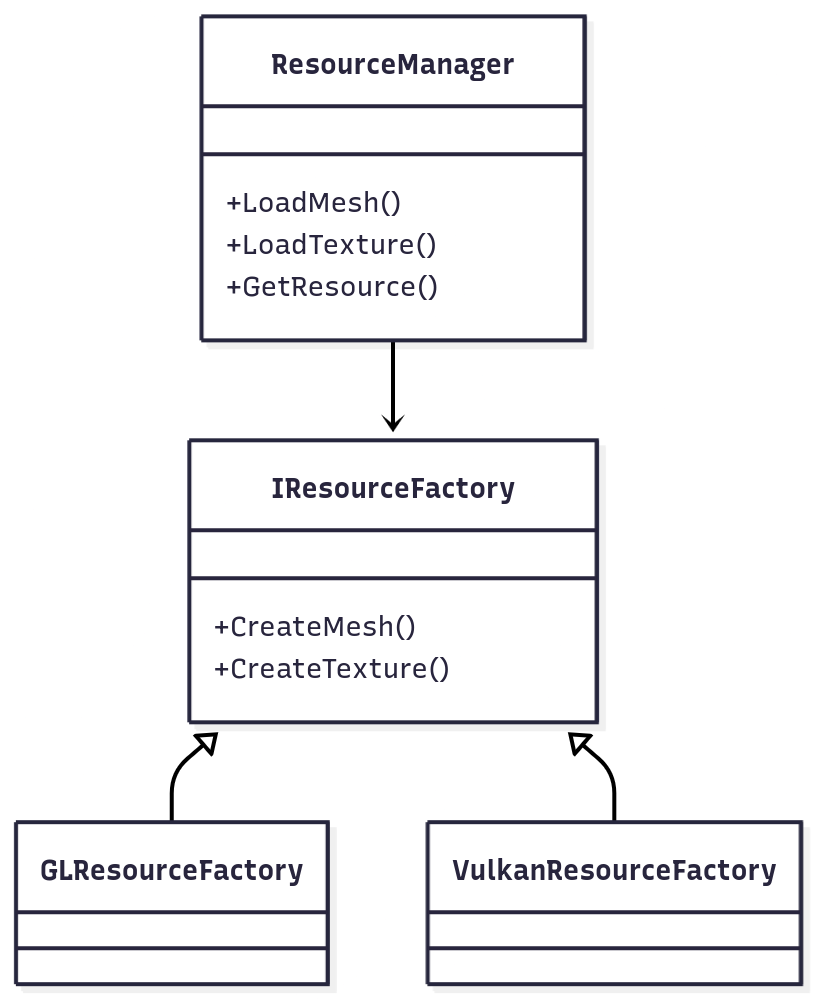
\includegraphics[width=.6\linewidth]{figures/uml_resources.png}
    \caption{Diagramma UML semplificato della gestione delle risorse.}
    \label{fig:uml-resources}
\end{figure}

%----------------------------------------------------------------------------------------
\chapter{Implementazione}
\label{chap:implementazione}
%----------------------------------------------------------------------------------------
\noindent
In questo capitolo viene descritto come le scelte progettuali presentate nel Capitolo~\ref{chap:design} sono state
effettivamente realizzate nel codice. L'obiettivo è illustrare la struttura del motore, le principali componenti
software, l'implementazione del sistema di materiali PBR, la simulazione di particelle e l'interfaccia grafica per
il monitoraggio delle prestazioni. Vengono inclusi frammenti di codice rappresentativi e diagrammi a supporto
della spiegazione.

\section{Struttura del Codice}
Il motore è organizzato in moduli distinti, separando il codice cross-API dalle implementazioni specifiche di OpenGL e
Vulkan. La struttura principale del progetto è la seguente:
\begin{itemize}
    \item \texttt{src/core}: codice indipendente dall'API, inclusi gestione della scena, materiali e componenti;
    \item \texttt{src/gl} e \texttt{src/vk}: implementazioni specifiche dei renderer e costrutti API specific;
    \item \texttt{resources/shaders/gl} e \texttt{resources/shaders/vk}: shader GLSL per ciascun backend;
    \item \texttt{resources/meshes} e \texttt{resources/textures}: asset 3D e texture utilizzate dal motore.
\end{itemize}
La compilazione è gestita tramite CMake, con opzioni per selezionare il backend grafico al momento del runtime:
\texttt{-g} per OpenGL e \texttt{-v} per Vulkan. Il motore può essere eseguito su Linux o Windows senza modifiche
al codice sorgente grazie all'uso di librerie multipiattaforma come GLFW e glm.

\section{Componenti Principali}
Il cuore del motore è costituito dai seguenti moduli:
\begin{itemize}
    \item \texttt{IRenderer}: interfaccia astratta che definisce le operazioni principali di inizializzazione,
          rendering e pulizia delle risorse.
    \item \texttt{GLRenderer} e \texttt{VulkanRenderer}: implementazioni specifiche per ciascun backend,
          incapsulando le complessità della gestione di buffer, pipeline e sincronizzazione.
    \item \texttt{Scene} e \texttt{Node}: organizzano gli oggetti in una gerarchia e gestiscono le trasformazioni.
    \item \texttt{ResourceManager}: carica, memorizza e gestisce mesh, texture e shader, utilizzando factory
          specifiche per OpenGL e Vulkan.
\end{itemize}

\section{Management della scena}
% TODO: Scene-Node relationship
% TODO: Parenting dei transform
% TODO: Components e component updates

\section{Management delle risorse}
% TODO: uid delle risorse
% TODO: Factory e metodi del manager?
% TODO: Material instance/material template

\section{Sistema di Materiali PBR}
Il motore implementa un sistema di materiali PBR basato sul modello Cook-Torrance. Ogni materiale è descritto
tramite \texttt{MaterialTemplate} e \texttt{MaterialInstance}, con parametri fisicamente plausibili come
roughness, metalness e albedo. Le informazioni vengono passate agli shader tramite uniform buffer (OpenGL) o
descriptor set (Vulkan).
La gestione dei materiali consente di applicare facilmente diversi set di texture PBR e modificare i parametri in
tempo reale tramite l'interfaccia grafica del motore.
% TODO: Oct-encoding
% TODO: Passaggio depth texture -> position lighting pass
% TODO: Snippet di parti del calcolo lighting PBR

\section{Simulazione di Particelle}
Il motore supporta sistemi di particelle configurabili tramite \texttt{ParticleSystemComponent}, con impostazioni
di emissione, fisica e rendering. Le particelle sono gestite come array di \texttt{ParticleInstanceData}, aggiornati
ogni frame. Il calcolo avviene su CPU in modo multithreaded, mantenendo compatibilità tra i due backend.
% TODO: Simple physics simulation (velocity/accel)
% TODO: Instanced rendering per le particelle

%----------------------------------------------------------------------------------------
\chapter{Valutazione delle Prestazioni}
\label{chap:valutazione}
%----------------------------------------------------------------------------------------

\section{Configurazione Sperimentale}

\section{Risultati}

\section{Discussione}

%----------------------------------------------------------------------------------------
\chapterWithoutNumber{Conclusioni e Sviluppi Futuri}
\label{chap:conclusioni}
%----------------------------------------------------------------------------------------

\paragraph{Sintesi del Lavoro}

\paragraph{Risultati Principali}

\paragraph{Limitazioni del Lavoro}

\paragraph{Sviluppi Futuri}

% End of thesis
\backmatter

\nocite{*}

\bibliographystyle{alpha}
\bibliography{bibliography}

% TODO: Write acknowledgements (optional)
\begin{acknowledgements}
   Optional. Max 1 page.
\end{acknowledgements}

\end{document}
